% !TeX program = xelatex
\documentclass[10pt,a4paper]{article}

\usepackage{polyglossia}
\setdefaultlanguage{hindi}
\newfontfamily\devanagarifont[Script=Devanagari]{Eczar}
\setotherlanguages{english}

\usepackage{tikz}
\usetikzlibrary{positioning, arrows, shapes.geometric}
\usepackage{graphicx}
\usepackage{caption, copyrightbox}
\usepackage{amsmath}
\usepackage{circuitikz}
\usepackage{subfig}
\usepackage{siunitx}
\usepackage{xfrac}
\usepackage[parfill]{parskip}
\usepackage{xcolor}
\usepackage[nottoc,numbib]{tocbibind}
\usepackage{lmodern}

\usepackage[hidelinks]{hyperref}
\hypersetup{
	pdftitle={Dhadak - A Pulse Oximeter},
	pdfsubject={Engineering, Circuit Design, Medical},
	pdfauthor={Y S K Abhijeet},
	pdfkeywords={oximeter, circuit design, electronics, heart rate}
}


\usepackage{pgfplots}
\pgfplotsset{compat=1.15}
\renewcommand\UrlFont{\ttfamilylatin}

\begin{document}
	
	\pagenumbering{roman}
	\begin{titlepage}
		\vspace*{5cm}
		{\centering
			
			
\includegraphics[width=1\textwidth]{../common/logo.png}\par
		}
		\vspace{4cm}
		\hfil \Large\bfseries हिन्दी \hfil
		\vfill
	\end{titlepage}
	
	भारत में COVID-19 की लहर के दौरान, मैंने देखा, बहुत लोग घर पर ऑक्सीजन के स्तर की निगरानी के लिए मेडिकल स्टोर और ऑनलाइन ऑक्सीमीटर खरीद रहें थे। मैं काफ़ी उत्सुक था, यह जानने के लिये कि उंगली से जुड़ा यह छोटा उपकरण हृदय गति और ऑक्सीजन संतृप्ति की गणना कैसे कर सक़ता है? इस सवाल ने मुझे शोध करने और समझने को प्रेरित किया कि वास्तव में ऑक्सीमीटर कैसे काम करता है और क्या मैं इसे खुद पुरा बना सक़ता हूं। इस प्रक्रिया में मुझे एहसास हुआ, सभी विवरणों को एक समझ दस्तावेज़ में लिखना सही होगा जो मेरे लिए एक स्मृति के रूप में काम करेगा और दूसरों के लिए भी मददगार हो सक़ता है।
साथ ही, मैं \LaTeX \hspace{1pt} सीखना शुरू करना चाहता था ताकि भविष्य की सभी परियोजनाओं के लिए सुंदर लिखित दस्तावेज़ तैयार किये जा सके।\bigskip

इस लेखन मे, ऑक्सीमीटर क्या है, ऑक्सीजन संतृप्ति और हृदय गति प्राप्त करने के लिए इलेक्ट्रॉनिक सर्किट का उपयोग कैसे किया जा सक़ता है, इसका एक संक्षिप्त सिद्धांत प्रस्तुत करने का प्रयास किया गया है। आवश्यक सर्किट तत्वों और ऐल्गोरिद्म पर भी चर्चा की गई है। यह माना गया है कि पाठक को निम्नलिखित विषयों का ज्ञान हैै:

\begin{itemize}
	\item बुनियादी सर्किट विश्लेषण \& इलेक्ट्रॉनिक तत्व
	\item ऑप एंप \& ट्रांजिस्टर के नियम
\end{itemize}

\bigskip

मैं इलेक्ट्रॉनिक्स सीखने कि यात्रा में नौसिखिया हूं, इसलिए इस लेख में गलतियां हो सकती हैं। प्रस्तुत जानकारी की सत्यता की जांच मेरे अलावा किसी अन्य व्यक्ति ने नहीं की है।
यह लेख इसलिए लिखा गया था ताकि ज्ञान का स्रोत बन सके कि ऑक्सीमीटर कैसे बनाया जाता है या ऑक्सीमीटर कैसे काम करता है। प्रस्तुत डिज़ाइन का उपयोग किसी भी जीवन समर्थन प्रणाली में नहीं किया जाना है।

\bigskip
यह दस्तावेज़ TexStudio editor मे लिखा गया है।	

सभी चित्र Inkscape से तैयार किए गए है।

लेखाचित्र GNU Octave मे बनाये गये है।

PCB \& Schematics को Kicad मे डिज़ाइन किया गया है।

एन्क्लोज़र FreeCAD मे डिज़ाइन किया गया है।

\medskip
परियोजना से संबंधित सभी फाइलें यहां है: \url{https://github.com/yskab/dhadak}

वीडियो श्रंखला: youtube.com/

\medskip
यदि कोई गलतियां मिलती है या सुधार करना चाहते हैं तो कृपया Github पर संपर्क करें। 

\medskip
पोस्ट और संदेशों के लिए Twitter पर मुझ तक पहुंच सकते हैं 
\href{https://twitter.com/yskabhijeet}{@yskabhijeet}


\includegraphics[width=0.2\textwidth]{../common/cc.png}\par

\vfill
\hfill
{\Large\bfseries वाई एस के अभिजीत}\par
\hfill
\large \today
	\tableofcontents
	\pagebreak
	\pagenumbering{arabic}
	
		
\section{Introduction}

	Oximetry is the process of measuring the concentration of oxygen in blood (oxygen saturation - SpO\textsubscript{2}). Normal levels of SpO\textsubscript{2} should usually be around 95\% to 100\%, level below 90\% could lead to Hypoxemia which can cause shortness of breath and headache\footnote{\url{https://www.mayoclinic.org/symptoms/hypoxemia/basics/definition/sym-20050930}}.

\subsection{Cardiac Cycle}

	Red blood cells contain Hemoglobin, a protein which when comes in contact with fresh oxygen via lungs forms Oxygenated Hemoglobin (HbO\textsubscript{2}). This Oxygenated blood is carried from the lungs to left side of the heart, which pumps this blood around the body through arteries. The cells of the body convert the chemical energy from oxygen molecules in red blood cells into Adenosine Triphosphate (ATP). ATP is stored in the cell and can be used for organism's life support system as required. Absence of oxygen in red blood cells due to conversion into ATP forms Deoxygenated Hemoglobin (Hb).\medskip

	This deoxygenated blood returns through the veins to right side of the heart, from there the blood is pumped into lungs to expel carbon dioxide and again fresh oxygen is inhaled and blood gets oxygenated. This completes a single Cardiac Cycle.

\subsection{Oximetry Principle}

	Pulse Oximeter is based on PPG (Photoplethysmography) wherein a light source is projected and a detector is used to measure volumetric changes in blood. It has been observed that Hb has a higher absorption when red wavelength is passed through while HbO\textsubscript{2} has a higher absorption towards infrared wavelength source (Figure \ref{fig:spectrum}). If we can relate the detected output with concentration of Hb/HbO\textsubscript{2} in blood, a relation can be obtained to calculate SpO\textsubscript{2}.

	\begin{figure}[ht!]
		\centering
		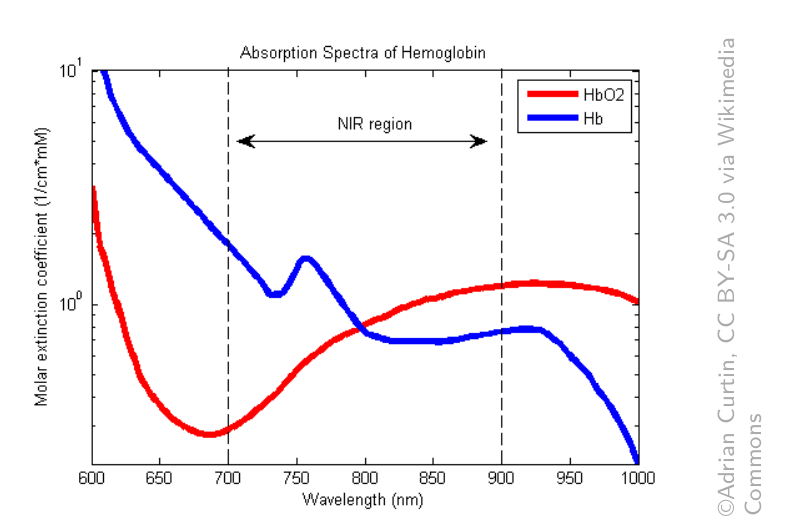
\includegraphics[width=0.7\textwidth]{../common/spectra.png}
		\caption{Absorption Spectra - Hb/HbO\textsubscript{2}}
		\label{fig:spectrum}
	\end{figure}
	
	
	\begin{figure}[ht!]
		\centering
		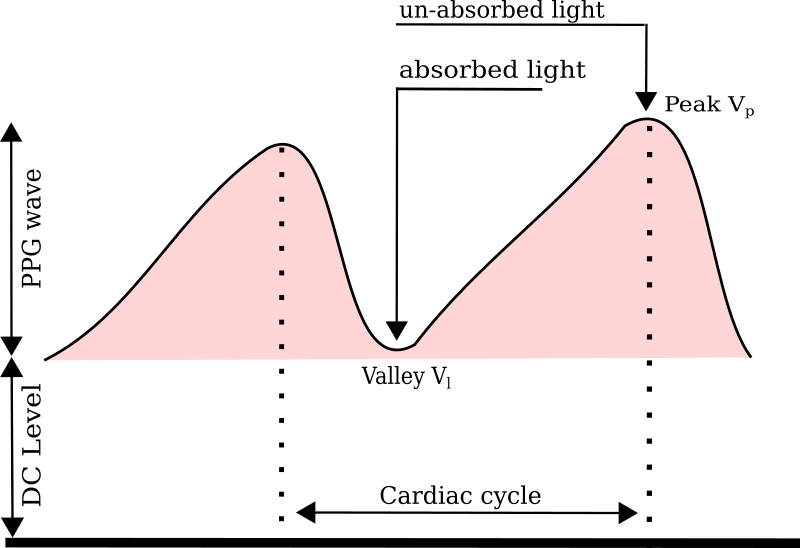
\includegraphics[width=0.7\textwidth]{images/PPG.png}
		\caption{PPG waveform when a single light source is projected}
		\label{fig:ppg}
	\end{figure}

	Heart pumps blood with each cardiac cycle and this leads to change in blood volume in the artery. When light is passed through (finger, earlobe, wrist\cite{light} depending on it's wavelength, Hb/HbO\textsubscript{2} components will also get absorbed and PPG signal is obtained as an output. Signal peaks correspond to completion of a cardiac cycle (heart beat). This varying signal also has a DC level due to absorption of light source by skin, venous blood and tissue.

	From this understanding, if we can find molecular concentrations of Hb and HbO\textsubscript{2} in a defined blood volume, SpO\textsubscript{2} can be calculated as a ratio of oxygenated blood concentration to total concentration: 

	\begin{equation}
		SpO\textsubscript{2} = \frac{HbO\textsubscript{2}}{Hb + 	HbO\textsubscript{2}}
	\end{equation}
	
	According to Beer-Lambert law:
	
	\begin{equation}		
		\log_{10}\frac{I}{I_o} = \epsilon l c
	\end{equation}	
	
	$I -$ Transmitted light intensity
	
	$I\textsubscript{o}-$ Incident light intensity
	
	$l -$ length
	
	$c -$ Molecular concentration
	
	$\epsilon -$ Molar absorption coefficient


	\begin{figure}[ht!]
		\centering
		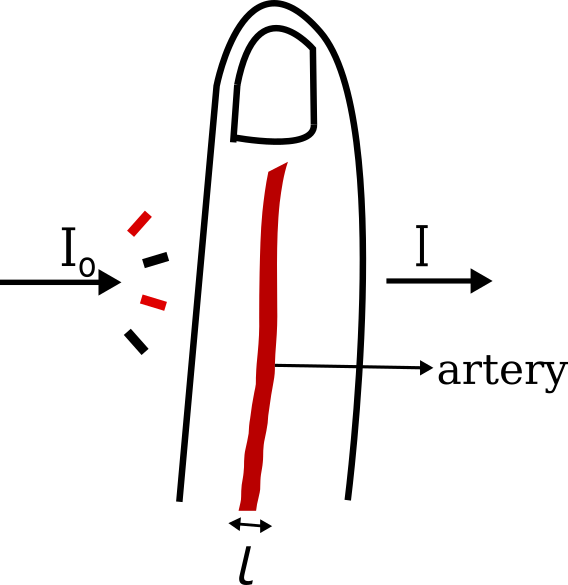
\includegraphics[width=0.3\textwidth]{images/finger_en.png}
		\caption{Light source projected onto a finger}
		\label{fig:finger}
	\end{figure}
	
	As seen in Figure \ref{fig:finger}, a light source is projected onto a finger and transmitted light is detected on the other end. Infrared and Red light is pulsed individually. For infrared source:
	
	\[	
	c_1 = 	\frac{\log_{10}\frac{I_1}{I_{o1}}}{\epsilon_1 l}
	\]	
	
	Since HbO\textsubscript{2} has higher absorption for infrared wavelength,

	\[	
	HbO_2 = \frac{\log_{10}\frac{I_1}{I_{o1}}}{\epsilon_1 	l}
	\]	
	
	Similarly for red,
	\[	
	Hb = \frac{\log_{10}\frac{I_2}{I_{o2}}}{\epsilon_2 	l}
	\]
	
	According to (1),

	\[	
	SpO_2 =  \frac{\frac{\log_{10}\frac{I_1}{I_{o1}}}{\epsilon_1 l}}		
	{\frac{\log_{10}\frac{I_2}{I_{o2}}}{\epsilon_2 l} + 	\frac{\log_{10}\frac{I_1}{I{o1}}}{\epsilon_1 l}}
	\]	
	
	if $R = \frac{\log_{10}\frac{I_2}{I_{o2}}}{\log_{10}\frac{I_1}{I_{o1}}}$,
	
	\[	
	SpO_2 = \frac{\frac{1}{\epsilon_1}}{\frac{R}{\epsilon_2} + \frac{1}{\epsilon_1}}
	\]	
	
	\begin{equation}
		SpO_2 = \frac{\epsilon_2}{R\epsilon_1 + \epsilon_2}
	\end{equation}	


	SpO\textsubscript{2} mostly depends on R, we can consider calculating R and later comparing with a calibrated reference to get the actual SpO\textsubscript{2}.
	
	Since Incident light intensity level would be constant while pulsed, R would depend only upon I\textsubscript{1} and I\textsubscript{2},

	\[
	R \approx \frac{\log_{10}{I_2}}{\log_{10}{I_1}} \approx \frac{I_2}{I_1} \approx \frac{AC_2}{AC_1}
	\]		
	
	We need not calculate the logarithm, as the actual SpO\textsubscript{2} would be obtained from a Look up table or an empirical equation which demonstrates relation of R to SpO\textsubscript{2}. Standard oximeter manufacturers would test their device on large group of subjects and obtain the R values and subject's actual SpO\textsubscript{2} using a separate calibrated meter to prepare a relationship curve. Once this mapping is obtained, SpO\textsubscript{2} for any subject can be calculated using the relationship.
	
	\begin{figure}[ht!]
	\centering	
	\begin{tikzpicture}
		\begin{axis}[
			xlabel = R,
			ylabel = SpO\textsubscript{2}\%]
			\addplot coordinates {
				(0.4, 100)
				(1, 85)
				(1.5, 72.5)
				(2, 60)
				(2.5, 47.5)
				(3, 35)
				(3.5, 22.5)
				(4, 10)
				(4.4,0)
			};
			
		\end{axis}
	\end{tikzpicture}
	\caption{A typical relationship curve R vs SpO\textsubscript{2}}
	\label{fig:curve}
	\end{figure}

	Since detected IR and Red signals can have varying DC levels, we need to normalize the ratio first by dividing the DC levels so that a direct comparison of the PPG (AC component) can be performed as that caries the absorbed/un-absorbed information, hence R now becomes:

	\[
		R = \sfrac{\frac{AC_2}{DC_2}}{{\frac{AC_1}{DC_1}}}
	\]	
	
	\begin{figure}[ht!]
		\centering
		\subfloat[Before Normalization
		]{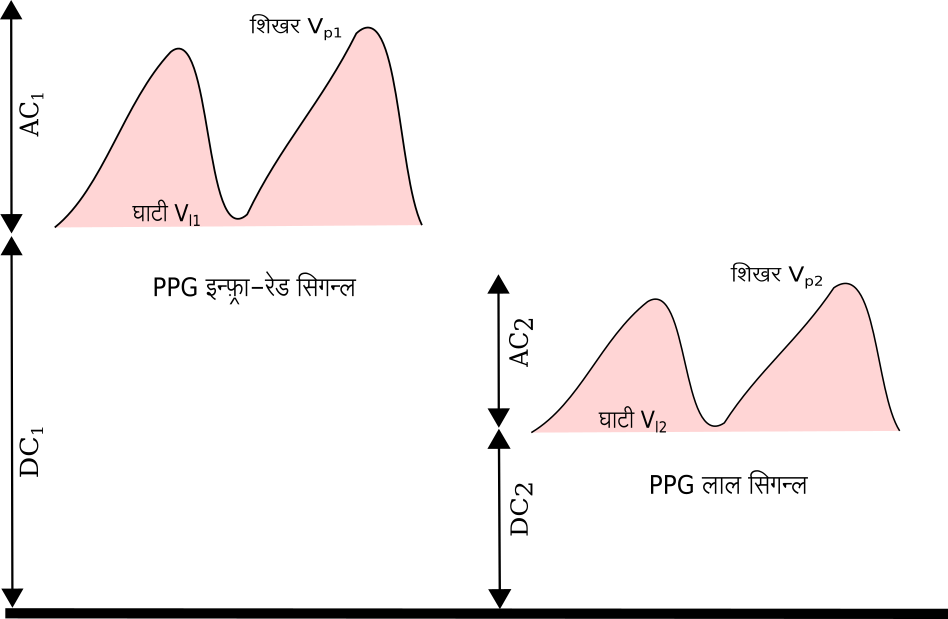
\includegraphics[width=0.7\textwidth]{images/PPG_norm1.png}}
		\hfill
		\subfloat[After Normalization
		]{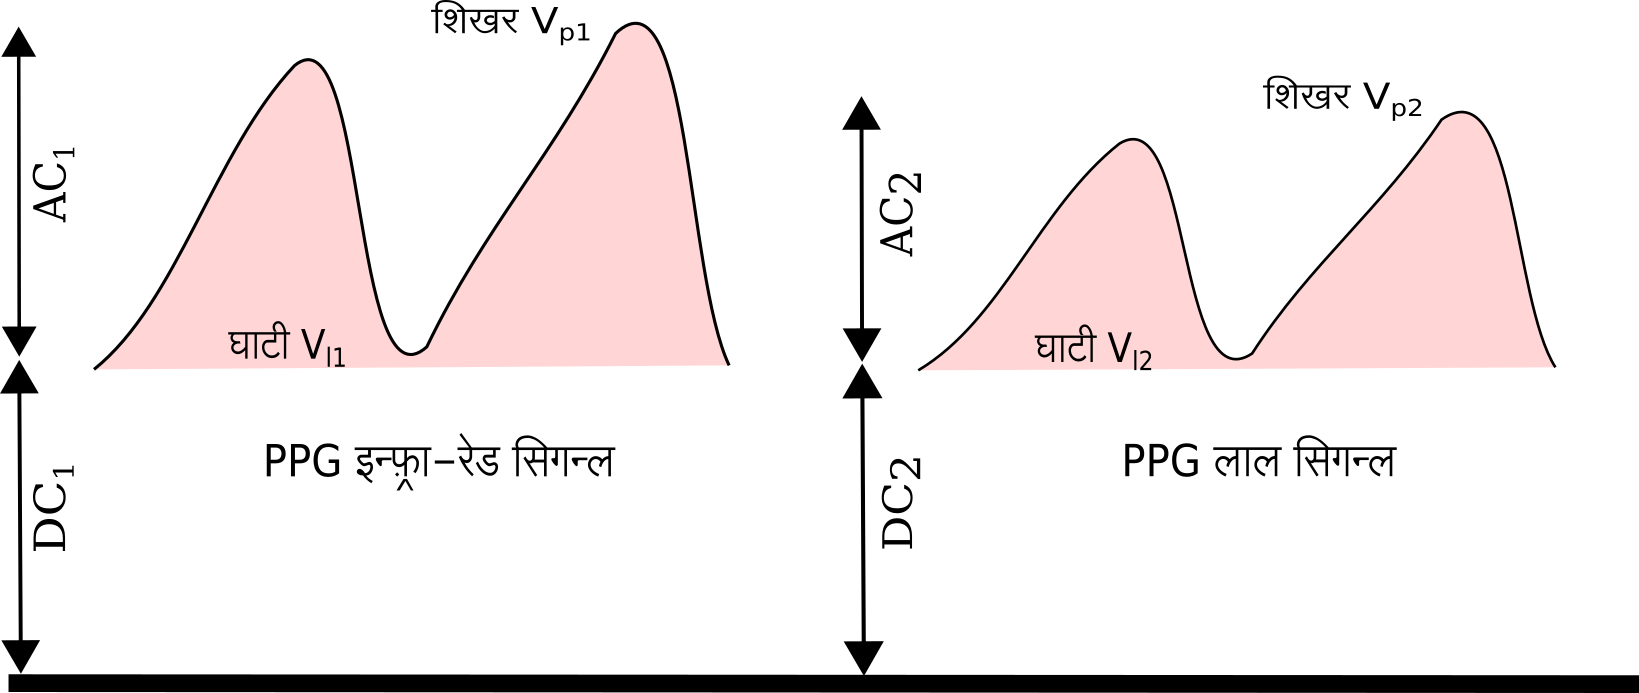
\includegraphics[width=0.7\textwidth]{images/PPG_norm2.png}}
		\caption{Effect of Normalization}
		\label{fig:ppgnorm}
	\end{figure}

	\begin{equation}
	\label{eq:calc}	
	R = \sfrac{\frac{V_{p2} - V_{l2}}{DC_2}}{\frac{V_{p1} - V_{l1}}{DC_1}}
	\end{equation}	 

	As shown in Figure \ref{fig:ppgnorm},
	
	$V_{p1} - $  Ir Peak
	
	$V_{l1} - $  Ir Valley
	
	$V_{p2} - $  Red Peak
	
	$V_{l2} - $  Red Valley
	
	$DC_1 - $  Ir DC level
	
	$DC_2 - $  Red DC level


	This value of R when compared with relationship curve would give the actual SpO\textsubscript{2}.
	
	We can consider calculating R for a set of samples and average them, instead of
	waiting for peaks and valleys to arrive. In this implementation, R is calculated between neighboring samples and a weighted average{\cite{wuk}} is calculated for final value. This is discussed further in SpO\textsubscript{2} calculation algorithm section.	
	\section{Main System Components}
	


	\subsection{Photodiode}
	
		Photodiode will be used as a detector in a reflective configuration, wherein light is projected from one end using LEDs and photodiode is detecting light at the opposite end converting it to current. This current would be proportional to LEDs brightness.
		
		
		\begin{figure}[ht!]
			\centering
			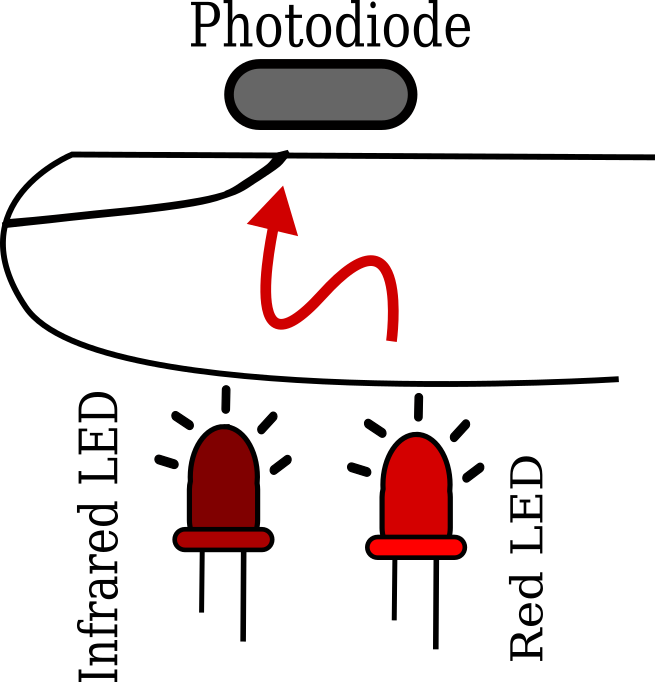
\includegraphics[width=0.3\textwidth]{images/finger_setup_en.png}
			\caption{Reflective finger setup}
		\end{figure}

		Photodiode needs to be sensitive in both red (700nm) and infrared (900nm) regions. QSB34CGR was used in this design which can work in both regions as seen in the sensitivity graph from part's datasheet.
	
		\begin{figure}[ht!]
			\centering
			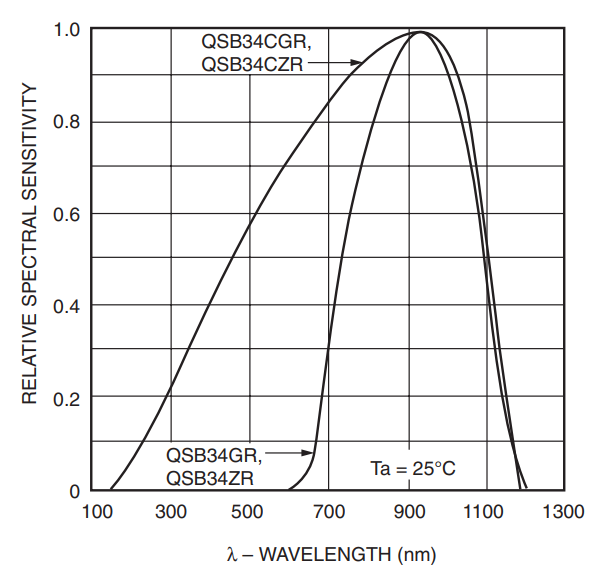
\includegraphics[width=0.6\textwidth]{../common/QSBCGR.png}
			\caption{QSB34CGR sensitivity spectrum}
		\end{figure}
	
	\pagebreak
	
	\subsection{Microcontroller}
	
		Microcontroller($\mu$C) is responsible for the algorithm in calculating the SpO\textsubscript{2} by reading the red and ir amplified channels via ADC. Also it performs the following tasks:
		
		\begin{itemize}
			\item Interfaces with an OLED 128x64 display to show the calculated  SpO\textsubscript{2} and heart beat.
			
			\item Interfaces with DACs.
		\end{itemize}
		
		Atmega4808 is used in this design.
	
	\subsection{Dual DAC}
	
		Dual digital to analog converter - MCP47FEB02A0 was used in design.
		
		\begin{itemize}
			
			\item DAC1 is required in LED driver stage so that $\mu$C can instruct the DAC to generate a required control voltage to set led current.
			
			\item DAC2 provides an input to the difference amplifier stage for DC removal from signals.
		
		\end{itemize}
		
	\subsection{Leds}
		It is important to select good leds for illumination, following factors ensure good signal response:
		
		\begin{itemize}
			\item Narrow view angle for less dispersion and deeper penetration into skin.
			\item Rectangular package in clear lens so that finger can rest comfortably.
			\item High radiant power.
		\end{itemize}
	
		I didn't get new leds and worked with generic 3mm/5mm ir led in circular clear package and a red led in diffused package. This caused the R ratio to not be correct. As a healthy individual, i was getting readings of R to be around 0.6 while it should be around 0.4. So I had to use a scaling factor to adjust the algorithm. A comment has been added in the program code regarding this. 
		
		A suitable choice can be Vishay Semiconductor's VSMD66694.
	
		  
	
	\section{सर्किट डिज़ाइन}
	\begin{figure}[ht!]
	\begin{tikzpicture}
		[->,>=stealth',semithick]	
		\node[rectangle,draw] (r0) at (0, 0) {फोटोडायोड};
		\node[rectangle,draw,text width=1cm, align=center] (r1) at (-1, -2) {लाल LED};
		\node[rectangle,draw,text width=1cm, align=center] (r2) at (1, -2) {इन्फ़्रारेड LED};	
		\node[rectangle,draw,text width=1cm, align=center] (r3) at (0, -4) {LED चालक};
		\node[rectangle,draw,text width=3cm, align=center] (r4) at (4, 0) {ट्रांस्इम्पेडेंस एम्पलीफायर};
		\node[rectangle,draw,text width=2cm, align=center]  (r5) at (8, 0) {डिफ़ैंस एम्पलीफायर};
		\node[rectangle,draw,text width=2cm, align=center] (r6) at (8, -2) {प्रोग्रामेबल गेन एम्प्लिफायर};
		\node[rectangle,draw,text width=3cm, align=center] (r7) at (8, -4) {$\mu$C ADC};
		\node[rectangle,draw,text width=1cm, align=center] (r8) at (2, -4) {$\mu$C};
		\node[rectangle,draw,text width=1cm, align=center] (r9) at (5, -2) {$\mu$C};
		
		\path (r1) edge (r0);
		\path (r2) edge (r0);
		\path (r3) edge (r1) 
		edge (r2);
		\path (r0) edge (r4);
		\path (r4) edge (r5);
		\path (r5) edge (r6);
		\path (r6) edge (r7);
		\path (r8) edge (r3);
		\path (r9) edge (r6);
		
	\end{tikzpicture}
	\caption{सिस्टम ब्लॉक आकृति}
	\end{figure}

	ब्लॉक आकृति का जिक्र करते हुए, उपखंड नीचे विभाजित हैं जो सर्किट और संबंधित आसिलोस्कोप ट्रेस आउटपुट दिखाते हैं।
	
	\subsection{फ्रंट एंड}	
	
		\subsubsection{ट्रांस्इम्पेडेंस भाग}
		
			फोटोडायोड के करंट को आनुपातिक वोल्टेज में बदलने की आवश्यकता होती है ताकि अंततः माइक्रोकंट्रोलर SpO\textsubscript{2} की गणना के लिए ADC का उपयोग करके वोल्टेज को डिजिटल मान में परिवर्तित कर सके। इसे प्राप्त करने के लिए एक साधारण ट्रांजिम्पेडेंस एम्प्लीफायर कॉन्फ़िगरेशन का उपयोग किया गया हैं:
			
			
			\begin{figure}[ht!]\centering
				\begin{circuitikz}[american] 
					\draw
					
					(2,3) node[op amp,yscale=-1] (opamp) {}
					(opamp.down) -- +(0,0.3) node[vcc]{Vcc}
					(opamp.up) -- +(0,-0.3) node[ground]{}
					(0,0) node[ground]{} to[pDo, l^=$D$, f^=$I$]  (0,2.5) to (opamp.-)
					(opamp.+) node[ground]{}
					(opamp.-) -- ++(0,-1.7) -- ++(0.5,0)
					to [R, l^=$R_1$] ++(1.5,0) -- ++(0.4,0) to (opamp.out)
					(opamp.-)  ++(0,-1.7) -- ++(0,-1.3) -- ++(0.5,0) 
					to [C, l^=$C_1$]  ++(1.5,0) -- ++(0.4,0) -- ++(0,1.3) 
					(opamp.out) -- ++(1,0) to [open,v=$V_1$,o-o] ++(0,-3) node[ground]{};
					
				\end{circuitikz}
			\end{figure}
			
		
			Led की तीव्रता के अनुसार, यदि फोटोडायोड में 10$\mu$A का करंट उत्पन्न होता है, और R = 100K$\Omega$, ओम के नियम के अनुसार, $V_1$ = 1 V। 
			कैपेसिटर का उपयोग पल्स कि लो-पास फ़िल्टरिंग के लिए किया जाता है। कट ऑफ आवृत्ति होगी:
		
			\begin{equation}	
				F_c = \frac{1}{2\pi R_1C_1}
			\end{equation}
			
			यदि R\textsubscript{1}=576K$\Omega$, C\textsubscript{1} = 33pF, 

			\[	
			F_c \approx \SI{8.3}{\kilo\hertz}
			\]
			
			\begin{figure}[ht!]
				\centering
				\subfloat[V\textsubscript{1} 
				]{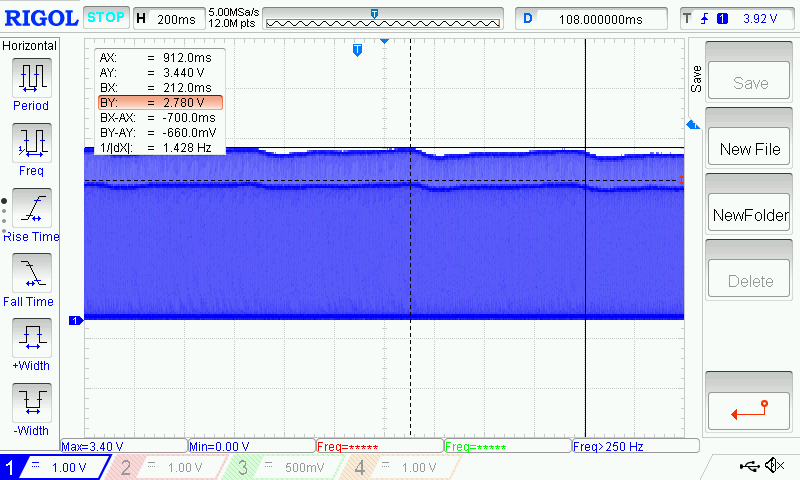
\includegraphics[width=0.9\textwidth]{../common/circuit/itov.png}}
				\hfill
				\subfloat[V\textsubscript{1} ज़ूम 
				]{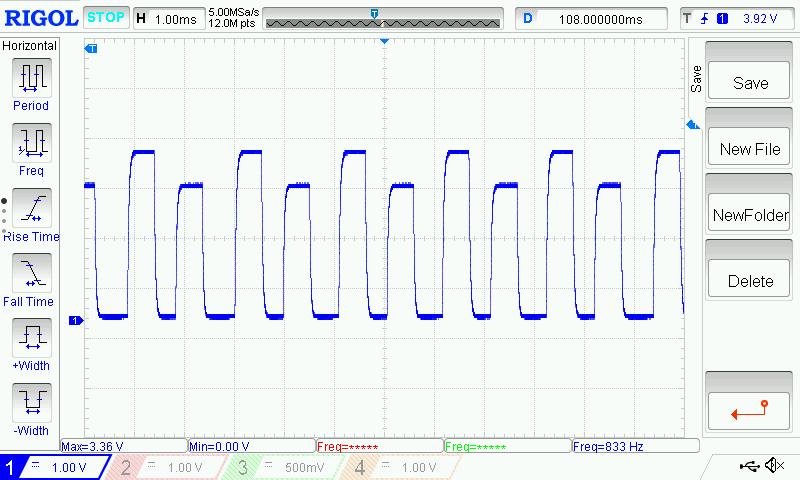
\includegraphics[width=0.9\textwidth]{../common/circuit/itov_zoom.png}
				\label{fig:itov}}
				\caption{V\textsubscript{1} ऑसिलोस्कोप ट्रेस (लाल \& इन्फ़्रारेड क्रमिक रूप से स्पंदित) }
			\end{figure}
			
			चूंकि led क्रमिक रूप से तेज दर के साथ ऑन-ऑफ होते हैं, इसलिए पल्स एक वर्ग तरंग की तरह दिखाई देगा। हमें led को स्पंदित करने के लिए इस कट-ऑफ के 1/10\textsuperscript{th} से कम पल्स फ्रीक्वेंसी का उपयोग करने होगा ताकि इसके सभी उच्च-आवृत्ति घटकों के साथ वर्ग तरंग स्पष्ट रूप से दिखाई दे और फ़िल्टर न हो।
			
			\[	
			F_p = \SI{500}{\hertz}
			\]
					
			
			यह ट्रेस में देखा जा सकता है, डीसी स्तर के उपर 2 PPG सिग्नल मोजुद हैं।
			उच्च आयाम इन्फ़्ररेड स्पंदन का परिणाम है, जबकि निचला आयाम लाल का है। चूँकि चोटियाँ हृदय गति के अनुरूप होती हैं, ट्रेस अनुसार यह 1.42/सेकंड या 85BPM है। सिग्नल का निर्माण करने वाली व्यक्तिगत स्पंद को चित्र \ref{fig:itov} में देखा जा सकता है। ज्ञात रेड सिग्नल का आयाम इन्फ़्ररेड से कम है, इसके कारण है:
			
			\begin{itemize}
				
				\item इन्फ्रारेड कि जादा तीव्रता उच्च इन्फ़्रारेड करंट के कारण।
				\item फोटोडायोड की लाल संवेदनशीलता इन्फ्रारेड संवेदनशीलता का 80\% है। 
				\item इन्फ्रारेड त्वचा में लाल से अधिक गहराई तक प्रवेश करता है, इसलिए फोटोडायोड पर बेहतर इन्फ्रारेड प्रतिक्रिया दिखाई देती है\cite{penetrate}। 
				
			\end{itemize}		
		
			इसलिए एक उपयुक्त सिगनल प्राप्त करने के लिए आवश्यक हे led की तीव्रता को बढ़ाना ताकि PPG सिग्नल का आयाम उच्च हो सके।	
			
		\subsubsection{डिफ़ैंस एम्पलीफायर}
		
			PPG सिग्नल को उपयुक्त स्तर तक बढ़ाने की जरूरत है ताकि सिग्नल को बेहतर ढंग से डिजिटाइज करने के लिए पूर्ण पैमाने पर ADC रेंज का उपयोग किया जा सके। अभी, PPG सिग्नल का आयाम काफी कम है और डीसी स्तर अधिक है। $\mu$C  DC को पढ़ सकता हैं और आर मूल्य गणना के लिए स्टोर कर सकता हैं, हमें केवल AC भाग को बढ़ाना होगा जो सिग्नल का एक आवरण है। प्रत्यक्ष बढ़ोतरी से डीसी स्तर भी प्राप्त होगा, क्योंकि आवश्यक संकेत इसके ऊपर सवार है। यह ऑप एंप को संतृप्त करेगा और बढ़ोतरी स्तर की सीमा काफी कम होगी।
		 
			
			\begin{figure}[ht!]
				\centering
				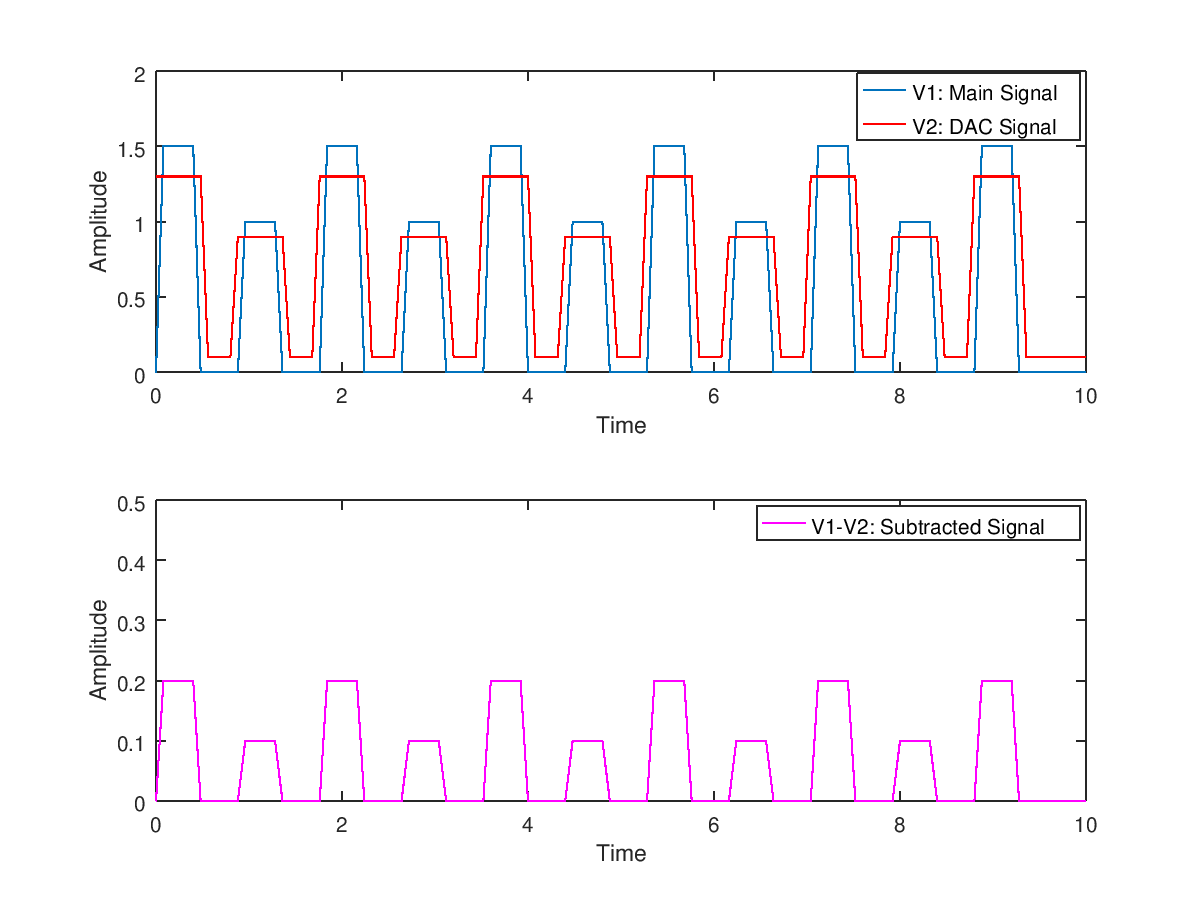
\includegraphics[width=0.8\textwidth]{../common/circuit/diff.png}
				\caption{डिफ़ैंस एम्पलीफायर का प्रभाव}
				\label{fig:diff}
			\end{figure}	
			
			यदि हम DC स्तर को पूरे सिग्नल से घटा सकें, तो केवल AC ही रहेगा जिसके स्तर को आसानी से आगे बढ़ाया जा सक़ता है। यह DC संकेत उत्पन्न करने के लिए 8 बिट डिजिटल से एनालॉग कनवर्टर (DAC) के साथ एक डिफ़ैंस एम्प्लीफायर का उपयोग यहां किया गया है। चूंकि लाल और इन्फ़्ररेड के अलग-अलग स्तर होते हैं, इसलिए DAC द्वारा स्पंदित आवृत्ति के अनुसार अलग-अलग डीसी स्तर उत्पन्न होते हैं।
			\medskip 
			
			जैसा कि चित्र \ref{fig:diff} में दिखाया गया है, Octave में उत्पन्न एक प्लॉट आवश्यक सिग्नल और डिफ़ैंस सिग्नल के घटाव को दर्शाता है। अब इस अंतर को और आगे बढ़ाया जा सक़ता है। डिफ़ैंस सिग्नल की पल्स चौड़ाई आवश्यक सिग्नल से थोड़ी बड़ी होती है ताकि आउटपुट सिग्नल में किनारों पर कोई स्पाइक न हो। डिफ़ैंस सिग्नल का निचला स्तर 0V से थोड़ा ऊपर है, जिससे अंतर हमेशा आवश्यक सिग्नल के 0V क्षेत्र में नकारात्मक हो और चूंकि ओप-अम्प एकल आपूर्ति पर परिचालन कर रहा है, इसलिए आउटपुट यहां 0V होगा।
			
			
			\begin{figure}[ht!]\centering
				\begin{circuitikz}[american] 
					\draw
					
					(4,3) node[op amp,yscale=-1] (opamp) {}
					(opamp.down) -- +(0,0.3) node[vcc]{Vcc}
					(opamp.up) -- +(0,-0.3) node[ground]{}
					(opamp.-) to [R, l^=$R_1$] ++(-2,0) node[label={left:$V_{dac1}$}] {}
					(opamp.+) to [R, l^=$R_1$] ++(-2,0) node[label={left:$V_1$}] {}
					(opamp.+) to [R, l^=$R_2$] ++(0,2) node[ground,rotate = 90]{}
					(opamp.-) -- ++(0,-1.7) -- ++(0.5,0)
					to [R, l^=$R_2$] ++(1.5,0) -- ++(0.4,0) to (opamp.out)
					(opamp.out) -- ++(1,0) to [open,v=$V_2$,o-o] ++(0,-3) node[ground]{};
			
				\end{circuitikz}
			\end{figure}
			

			\[
			V_2 = \frac{R_1}{R_1}(V_1 - V_{dac1})
			\]
			
			
			यदि, $R_1 = 10K$,
			
			\[
			V_2 \approx V_1 - V_{dac1}
			\]
		
			
		\subsubsection{प्रोग्रामेबल एम्पलीफायर}
		
			सिगनल को बढ़ाना आवश्यक हो जाता है क्योंकि त्वचा की टोन, सेंसर के साथ अनुचित उंगली संपर्क या किसी भी त्वचा रंजकता\cite{skin} से सिगनल में क्षीणन होता है। यह चरण चयन योग्य परिवर्तनीय लाभ प्रदान करता है जिसे माइक्रोकंट्रोलर द्वारा निर्धारित किया जा सक़ता है।
			
			$\mu$C निर्धारित करेगा कि किस स्तर के प्रवर्धन की आवश्यकता है और संबंधित सिगनल पिन को उच्च ड्राइव करेगा ताकि संबंधित अवरोध चयनित हो जाए।
			
			
			\begin{figure}[ht!]\centering
				\begin{circuitikz}[american] 
					\draw
						(2,3) node[op amp,yscale=-1] (opamp) {}
						(opamp.down) -- +(0,0.3) node[vcc]{Vcc}
						(opamp.up) -- +(0,-0.3) node[ground]{}
						(opamp.+) to ++(-2,0) node[label={left:$V_2$}] {}
						(opamp.-) -- ++(0,-1.7) -- ++(1,0)
						to [R, l^=$10K$] ++(1,0) -- ++(1,0) -- ++(0,2.2) to (opamp.out)
						(opamp.-) ++(0,-1.7) -- ++(0,-1.5) to [R, l^=$10K$] ++(0,-1) -- ++(0,-0.5)
						++(0,-0.5) node[npn] (Q1){}
						(Q1.E) node[ground]{}
						(Q1.B) to [R, l^=$4.7K$] ++(-1.5,0) node[label={left:S1}] {}
						
						(opamp.-) ++(0,-1.7) ++(0,-0.75) -- ++(3.5,0) -- ++(0,-0.75)		
						to [R, l^=$4.7K$] ++(0,-1) -- ++(0,-0.5)
						++(0,-0.5) node[npn] (Q2){}	
						(Q2.E) node[ground]{}	
						(Q2.B) to [R, l^=$4.7K$] ++(-1.5,0) node[label={left:S2}] {}
						
						(opamp.-) ++(0,-1.7) ++(0,-0.75) ++(2,0) -- ++(5,0) -- ++(0,-0.75)		
						to [R, l^=$2.35K$] ++(0,-1) -- ++(0,-0.5)
						++(0,-0.5) node[npn] (Q3){}	
						(Q3.E) node[ground]{}	
						(Q3.B) to [R, l^=$4.7K$] ++(-1.5,0) node[label={left:S3}] {};
						
						
				 \end{circuitikz}
			\end{figure}	
	
			\begin{center}
				\begin{tabular}{ |c|c|} 
					\hline
					\textbf{स्विच} & \textbf{बढ़त}   \\ 
					\hline
					सभी बंद & 1 	 \\ 
					\hline
					S1 & 2  		\\ 
					\hline
					S2 & 3  		\\ 
					\hline
					S1+S2 & 4  		\\ 
					\hline
					S3 & 5  		\\ 
					\hline
					S1+S3 & 6	  	\\ 
					\hline
					S2+S3 & 7  		\\ 
					\hline
				\end{tabular}
			\end{center}
	
	
	\subsection{LED चालक}

	
		जैसा कि पहले चर्चा की गई थी, ट्रांस्इम्पेडेंस चरण के बाद सिगनल स्तर बहुत कम हो सकता है। led ड्राइवर को आवश्यकतानुसार led के केरंट बढ़ाना की जरूरत है। निम्नलिखित सर्किट का उपयोग वोल्टेज नियंत्रित करंट स्रोत के रूप में किया गया है, वोल्टेज को DAC सेट करता है $\mu$C के निर्देशन पे।
		
		\begin{figure}[ht!]\centering
			\begin{circuitikz}[american] 
				\draw
				
				(4,3) node[npn] (Q1){}
				(Q1.E) to [R, l^=20] ++(0,-1.5) node[ground]{}
				(Q1.B) to [R, l^=4.7K] ++(-1.5,0) node[label={left:$V_{dac2}$}] {}
				(Q1.C) -- ++(-1,0) -- ++(0,0.5) ++(0,0.5)  node[npn] (Q2){}
				(Q2.B) to [R, l_=10K] ++(-1.5,0) node[label={left:Red pulse}] {}
				(Q2.C) -- ++(0,1) node[]{} ++(0,0.2) node[]{Red cathode}
				(Q1.C) -- ++(1,0) -- ++(0,0.5) ++(0,0.5) node[npn,xscale=-1] (Q3){}
				(Q3.B) to [R, l^=10K] ++(1.5,0) node[label={right:IR pulse}] {}
				(Q3.C) to ++(0,1) node[]{} ++(0,0.2) node[]{Ir cathode};
			\end{circuitikz}
		\end{figure}
		
		
		जब भी लाल/इन्फ्रारेड पल्स सक्रिय होता है, तो led एकल पुल विन्यास द्वारा सक्रिय हो जाते हैं, संबंधित लाल/इन्फ्रारेड led सक्रिय हो जाते हैं (Vcc से जुड़े led एनोड)। करंट की मात्रा $V_{dac2}$ \& $R_1$ पर निर्भर करेगी।
		
		$V_{dac2}$ भी स्पंदित आवृत्ति के अनुसार लाल और इन्फ़्रारेड के लिए अलग-अलग सेट किया जायेगा। यदि सिग्नल का पता लगाने के लिए तीव्रता पर्याप्त नहीं हो, तो $V_{dac2}$ को बढ़ाना आवश्यक है। $\mu$C थ्रेसहोल्ड का निर्धारण करेगा और उसके अनुसार नियंत्रण वोल्टेज को संशोधित करेगा।	

		प्रोग्रामेबल एम्पलीफायर चरण के बाद अंतिम आउटपुट नीचे दिखाया गया है। प्राप्त PPG सिग्नल - लाल और इन्फ़्ररा-रेड स्पष्ट रूप से दिखाई दे रहे है और एक उपयुक्त स्तर पर है जिसे ADC को भेजा जा सक़ता है ऐल्गोरिद्म मे उपयोग के लिये। 
	
	\begin{figure}[ht!]
		\centering
		\subfloat[अंतिम आउटपुट - हरा, V\textsubscript{1} - नीला
		]{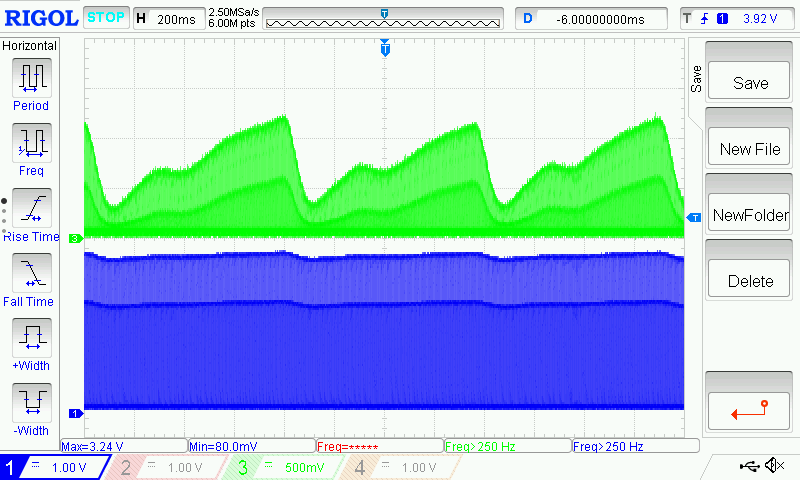
\includegraphics[width=1\textwidth]{../common/circuit/final_out.png}}
		\hfill
		\subfloat[अंतिम आउटपुट का माप
		]{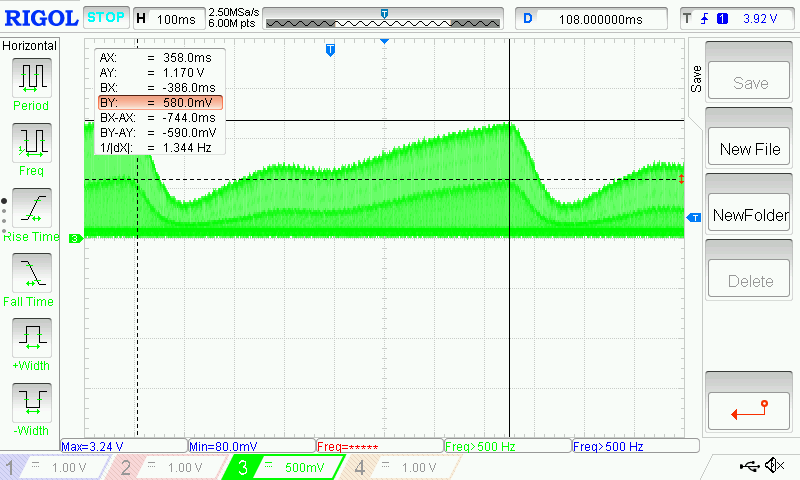
\includegraphics[width=1\textwidth]{../common/circuit/final_out_meas.png}}
		\caption{अंतिम आउटपुट}
	\end{figure}	
	
	\section{ऐल्गोरिद्म}
	
	\begin{figure}[ht!]
		\hspace*{-1.8cm}
		\begin{tikzpicture}
			[node distance=1.5cm]
			
			\tikzstyle{startstop} = [rectangle, rounded corners, minimum width=3cm, minimum height=1cm,text centered, draw=black, fill=pink!30,align = center]
			
			\tikzstyle{io} = [trapezium, trapezium left angle=70, trapezium right 	angle=110, minimum width=3cm, minimum height=1cm, text centered, draw=black]
			
			\tikzstyle{process} = [rectangle, minimum width=3cm, minimum height=1cm, text 	centered, draw=black,align = center, fill = blue!20]
			
			\tikzstyle{decision} = [diamond, minimum width=3cm, minimum height=1cm, 
			align = center, draw=black, fill = green!20]
						
			\tikzstyle{arrow} = [thick,->,>=stealth]

			\node (st) [startstop] {शुरु};
			\node (pls) [process,below of=st] {led पल्स शुरू};
			\node (wt) [process, below of=pls] {0.5 सेकंड प्रतीक्षा};
			\node (findlv) [decision, below of=wt,yshift=-1cm] {$V_1$ निर्धारित स्तर\\के अन्तर्गत};
			\node (setlv) [process, left of=findlv,xshift=-3cm] {नया ड्राइव करंट सेट करें};
			\node (dc) [process, below of=findlv,yshift=-1cm] {लाल/इन्फ़रा का \\DC स्तर खोजें};
			\node (diff) [process, below of=dc] {डिफ सिग्नल उत्पन्न करें};
			\node (amp) [decision, below of=diff,yshift=-1cm] {$V_2$ निर्धारित \\ स्तर के अन्तर्गत};
			\node (pga) [process, left of=amp,xshift=-3cm] {PGA: बढ़त चुन\\कर एम्प्लिफ़्य};
			\node (adc) [process, below of=amp,yshift=-1cm] {प्रत्येक पल्स पर\\ADC पढ़ें};
			\node (filt) [process, below of=adc] {$2^{nd}$ ऑर्डर IIR फ़िलटर};
			\node (peaks) [process, below of=filt] {शिखर - घाटी का \\पता लगाएं};
			\node (hr) [startstop,right of=peaks,xshift=+2.5cm] {HR की गणना};
			\node (ratio) [process,right of=filt,xshift=+2.5cm] {R अनुपात की गणना};
			\node (spo2) [startstop,right of=ratio,xshift=+2.5cm] {औसत $SpO_2$\& \\कि गणना};
			
			\draw [arrow] (st) -- (pls);
			\draw [arrow] (pls) -- (wt);
			\draw [arrow] (wt) -- (findlv);
			\draw [arrow] (findlv) -- node [above]{गलत} (setlv);
			\draw [arrow] (setlv) |- (pls);
			\draw [arrow] (findlv) -- node [left]{सही} (dc);
			\draw [arrow] (dc) -- (diff);
			\draw [arrow] (diff) -- (amp);
			\draw [arrow] (amp) -- node [above]{गलत} (pga);
			\draw [arrow] (amp) -- node [left]{सही} (adc);
			\draw [arrow] (pga) |- (adc);
			\draw [arrow] (adc) -- (filt);
			\draw [arrow] (filt) -- (peaks);
			\draw [arrow](peaks) -- (hr);
			\draw [arrow](filt) -- (ratio);
			\draw [arrow](ratio) -- (spo2);	
		
		
			\draw (pls) ++(3.6,0) node [align = left]{\footnotesize
			लाल$\backslash$इन्फ़्रारेड led क्रमिक\\
			\footnotesize रूप से चालु $\SI{500}{\hertz}$ पे};
			
			\draw (wt) ++(3.5,0) node [align = left]{\footnotesize
			0.5 सेकंड प्रतीक्षा PPG\\\footnotesize सिग्नल ठहराने के लिए};
			
			\draw (findlv) ++(3.7,0) node [align = left]{\footnotesize
			जाँचे PPG सिग्नल निर्धारित \\\footnotesize स्तर के अन्तर्गत नहीं तो\\
			\footnotesize नया ड्राइव करंट सेट करें};
			
			\draw (dc) ++(3.4,0) node [align = left]{\footnotesize
			लाल/इन्फ़रा DC स्तर \\\footnotesize खोजें डिफ़ सिगनल \\\footnotesize के लिये};
			
			
			\draw (diff) ++(3.6,0) node [align = left]{\footnotesize
			DAC डिफ़ सिगनल उत्पन्न \\\footnotesize करेगा DC घटाव के लिये};
			
			\draw (amp) ++(3.4,0) node [align = left]{\footnotesize
			PGA सक्षम करें यदि\\\footnotesize $V_2$ स्वीकार्य स्तर के \\\footnotesize भीतर नही हो};
			
			\draw (ratio) ++(0,1) node [align = left]{\footnotesize
				R कि गणाना\\\footnotesize पडोसी समंक बिन्दुओ से};
			\draw (spo2) ++(0,1) node [align = left]{\footnotesize
				मध्यवर्ती $SpO_2$ का\\\footnotesize औसत अंतिम मूल्य के लिए};
			
		\end{tikzpicture}
		\caption{योजना प्रवाह}
	\end{figure}
	
	\subsection{IIR फ़िलटर}

		ADC से पड़े सिगनल मे शोर हो सकता है, यदि यह सिगनल सीधे शिखर - घाटी की खोज मे प्रयोग कर दिया गया, तो बहुत सारी शिखर - घाटी सटीक रूप से नहीं मिलेगा शोर के कारण। इसलिये यह ज़रुरी है कि शोर को न्यूनतम करा जा सके। 
		एक 2\textsuperscript{nd} ऑर्डर IIR फ़िलटर सिगनल को सुचारु करने के लिए पर्याप्त है। अंतर समीकरण के रूप में 2\textsuperscript{nd} ऑर्डर IIR ट्रांसफर फ़ंक्शन नीचे दिया गया है:
		
		\[
		y_i = b_1*x_i + b_2*x_{i-2} - a_2*y_{i-1} + b_3*x_{i-1} - a_3*y_{i-2}
		\]
		
		जाहा,
		
		$y_i$: मौजूदा आउटपुट
		
		$y_{i-1}$: पिछला आउटपुट
		
		$y_{i-2}$: $y_{i-1}$ का पिछला आउटपुट
		
		$x_i$: मौजूदा इनपुट
		
		$x_{i-1}$: पिछला इनपुट
		
		$x_{i-2}$: $x_{i-1}$ का पिछला इनपुट
		
		\begin{figure}[ht!]
			\centering
			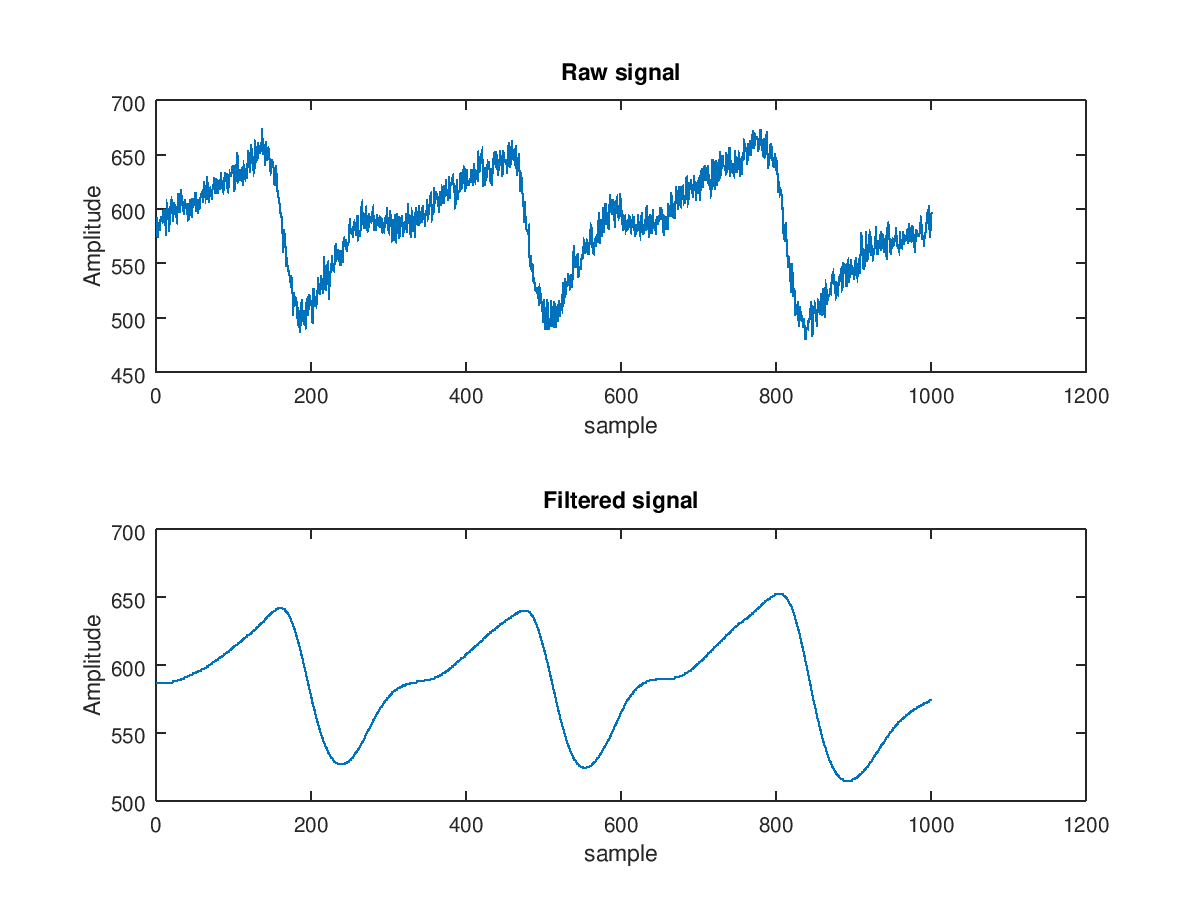
\includegraphics[width=0.8\textwidth]{../common/algo/filter.png}
			\caption{2\textsuperscript{nd} ऑर्डर बटरवर्थ IIR फ़िलटर}
			\label{fig:filter}
		\end{figure}
		
		Octave's $butter$ function\footnote{\url{https://octave.sourceforge.io/signal/function/butter.html}} का प्रयोग लो पास कॉन्फ़िगरेशन के लिए स्थानांतरण फ़ंक्शन गुणांक प्राप्त करने के लिए किया गया था।  Sampling आवृत्ति 500Hz और cut-off 3.3Hz (अधिकतम HR 200 के लिये) दिया गया था। गुणांक मान:
		
		$a_2 = -1.94137, a_3 = 0.94304$
		
		$b_1 = b_3 = 4.1762e-04$
		
		$b_2 = 8.3523e-04$	
		
		फ़िल्टर के प्रदर्शन को स्पष्ट करने के लिए, ADC से लाल सिग्नल लिया गया था, फ़िल्टर समीकरण लागू किया गया था Octave मे। जैसा कि चित्र \ref{fig:filter} में देखा गया है, फ़िल्टर शोर को दबाने में काफ़ी प्रभावी है और एक सहज आउटपुट\footnote{वास्तविक प्रोग्राम में केवल 1\textsuperscript{st} ऑर्डर फ़िल्टर लागू किया गया था क्योंकि वह अच्छा काम कर रहा था, लेकिन उपयुक्त फ़िल्टरिंग प्रदर्शन के लिए 2\textsuperscript{nd} ऑर्डर फ़िल्टर होना बहुत बेहतर है।} उत्पन्न करता है।
		
	
	\subsection{हृदय गति}
	
		हृदय गति गणना mountaineer's method for peak detection (MMPD)\cite{mmpd} ऐल्गोरिद्म से करी गयी है। 
		
		इस पद्धति में, प्रत्येक बिन्दु के लिए ढलान की गणना की जाती है और जैसे-जैसे ढलान सकारात्मक से ऋणात्मक में बदलता है, बिन्दु एक शिखर के अनुरूप होगा। इसी तरह एक ढलान का ऋणात्मक से सकारात्मक में परिवर्तन एक घाटी होगा। सकारात्मक या ऋणात्मक लगातार ढलानों के लिए एक गिनती भी ली जाती है और एक पूर्व निर्धारित मूल्य के साथ तुलना की जाती है जो ऐल्गोरिद्म की सुधार करने के लिए प्रत्येक ज्ञात शिखर के साथ अद्यतन होता है।
		
		एक टाइमर शिखर टाइमिंग को स्टोर करेगा और लगातार चोटियों के बीच समय का अंतर हृदय गति (HR) के अनुरूप होगा।
		
		\begin{figure}[ht!]
			\centering
			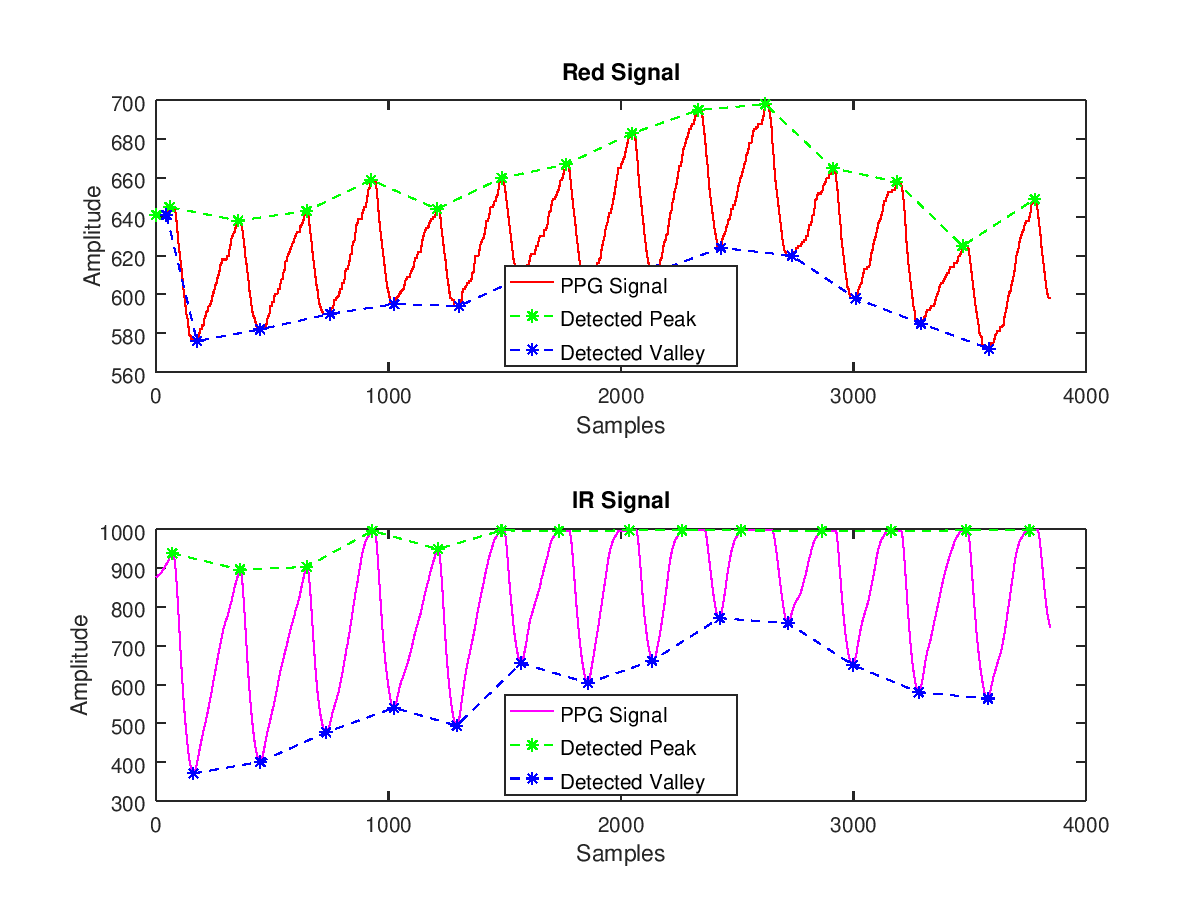
\includegraphics[width=0.7\textwidth]{../common/algo/mmpd.png}
			\caption{डेटा पर लागू ऐल्गोरिद्म}
		\end{figure}
	
	\subsection{SpO\textsubscript{2} गणना}
		
		जेसा कि पहले समीकरण \eqref{eq:calc} मे देखा गया हे:
		
		\[
			R = \sfrac{\frac{V_{p2} - V_{l2}}{DC_2}}{\frac{V_{p1} - V_{l1}}{DC_1}}
		\]	
		
		हम R कि गणना के लिए सिग्नल के वास्तविक शिखर और घाटियों का उपयोग नहीं करना चाहते हैं क्योंकि यह हृदय गति पर निर्भर है और यदि औसत निकाला जाये इस गणना से विभिन्न बिंदुओं के लिए तो अंतिम SpO\textsubscript{2}\% प्रपात करने में देरी होगी। इसलिए एक वज़न औसत विधि\cite{wuk} का उपयोग किया जाता है, जहां तात्कालिक SpO\textsubscript{2}\% की गणना पड़ोसी बिंदुओं के लिए की जाती है और एक साथ औसत करी जाती है। यह सुनिश्चित करता है कि कई तात्कालिक मूल्य प्राप्त होते हैं जिन्हें अंतिम मूल्य प्राप्त करने के लिए औसत किया जा सकता है। इस विधि मे निम्नलिखित चरणों को क्रम में किया जाता है:
		
		\begin{figure}[ht!]
			\centering
			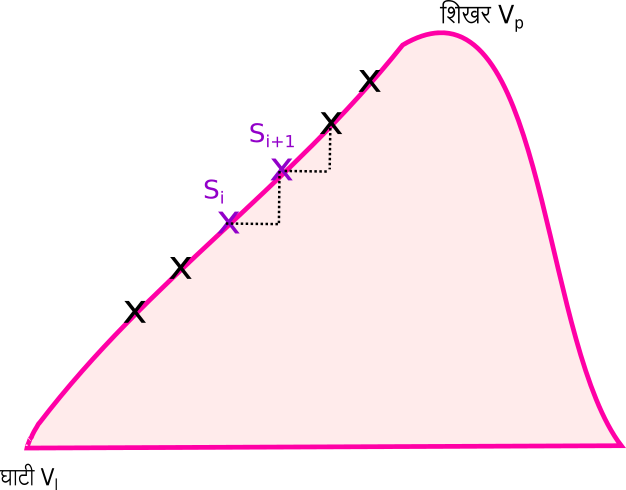
\includegraphics[width=0.5\textwidth]{images/spo2_algo.png}
			\caption{तात्कालिक SpO\textsubscript{2} के लिये चयनित बिन्दु}
		\end{figure}
	
		\begin{enumerate}
			\item लाल और इन्फ़्रारेड बिन्दुओ के क्रमागत नमूनों के बीच R प्रापत करना होगा: $S_{i+1}$ \& $S_{i}$. 
			
			\[
				R = \sfrac{\frac{S_{i_2+1} - S_{i2}}{DC_2}}{\frac{S_{i_1+1} - 		S_{i1}}{DC_1}}
			\]	
			
			इस R मान के साथ SpO\textsubscript{2} खोजें, जो एक विशिष्ट संबंध वक्र समीकरण का उपयोग करके प्राप्त किया जा सकता है जेसा कि चित्र \ref{fig:curve} मे देखा गया था:
			\[		
			SpO_2 = -25*R + 110;
			\]
			
			\item वर्तमान औसत के आधार पर इस SpO\textsubscript{2} को भार दें। यदि यह तात्कालिक SpO\textsubscript{2} औसत से कम है, तो कम भार निर्दिष्ट करें। यदि औसत के करीब है, तो अधिक भार निर्दिष्ट करें। 
			
			\item 20 बिन्दुओ के लिए भार सौंपे जाने के बाद, एक भारित औसत की गणना करें। इस भारित औसत को स्टोर करें।
			
			\item चरण 1 पर पुनरारंभ करें और ऐसे 10 पुनरावृत्तियों को निष्पादित करें।
			
			\item 10 पुनरावृत्तियों के बाद, प्रत्येक पुनरावृत्ति में परिकलित भारित औसत का औसत करे। यह अंतिम SpO\textsubscript{2} बन जाता है। इस मान को वर्तमान SpO\textsubscript{2} औसत से अपडेट करें जिसका उपयोग भार निर्दिष्ट करने के लिए किया जाता है।

		\end{enumerate}
	
		इस एल्गोरिथम का विस्तृत विवरण में मौजूद है - Pulse Oximetry: Analysis of Theory, Technology and Practise\cite{wuk}		
			
			
		अंत में, प्रत्येक 5 सेकंड में एक OLED डिस्प्ले पर SpO\textsubscript{2}\% और HR का मान प्रदर्शित किया जाता है।	
	\section{PCB \& Enclosure}

	\subsection{PCB}	
	
		\begin{figure}[ht!]
			\centering
			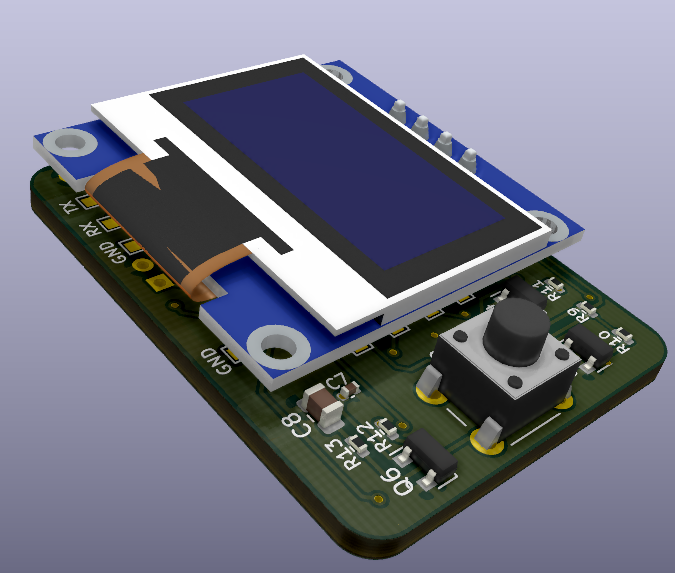
\includegraphics[width=0.6\textwidth]{../common/pcb/pcb.png}
			\caption{Completed PCB}
		\end{figure}


		\begin{figure}[ht!]
			\centering
			\subfloat[PCB Back
			]{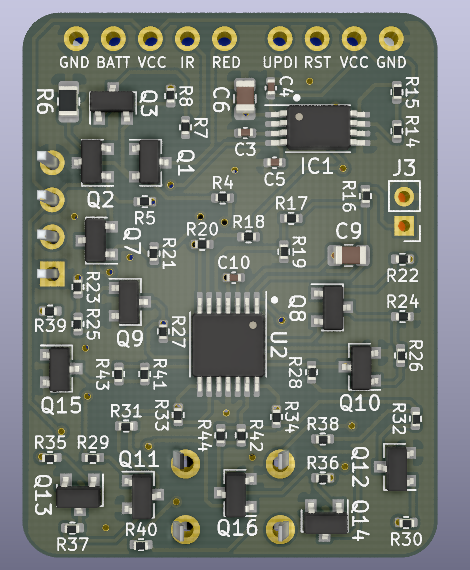
\includegraphics[width=0.5\textwidth]{../common/pcb/pcb_back.png}}
			\hfill
			\subfloat[PCB Front
			]{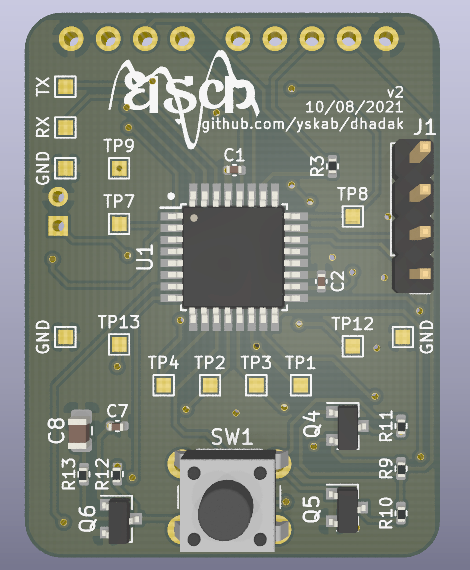
\includegraphics[width=0.5\textwidth]{../common/pcb/pcb_front.png}}
			\caption{PCB Images}
		\end{figure}

		PCB Design was completed on 2 layers with most of the components placed on the back side so that they can be re-flowed easily on a dosa pan. All components on front side are to be hand soldered.
		
		\begin{itemize}
			
			\item Design also includes a soft latch power on/off switch circuit to easily operate the device.
			
			\item A programming header was also added to program the $\mu$C via UPDI interface.
			
			\item Connection headers were added to connect the leds, battery \& photodiode which will be present on bottom compartment of enclosure.
			
			\item Header to attach OLED Display.

		\end{itemize}
	
		Sufficient test points were added on front side for easy access to probe and view the signals on oscilloscope.
		
		To keep the PCB size equivalent to that of the OLED display module, 0402 size resistors/capacitors were used.
			

	\subsection{Enclosure}		
		
		Enclosure was designed taking reference from a typical Oximeter which has display \& PCB on top, a finger insert below and a bottom part with battery compartment.
		
		\begin{figure}[ht!]
			\centering
			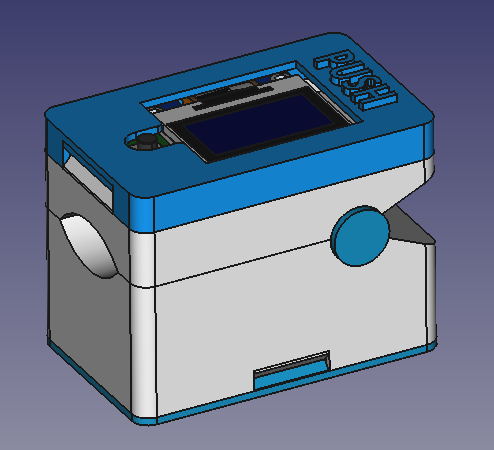
\includegraphics[width=0.5\textwidth]{../common/enc/enc.png}
			\caption{Completed Enclosure}
		\end{figure}	
		
				
		A reflective setup was implemented with photodiode on top base and pulse leds in bottom compartment. 
				
		\begin{figure}[ht!]
			\centering
			\subfloat[Photodiode compartment
			]{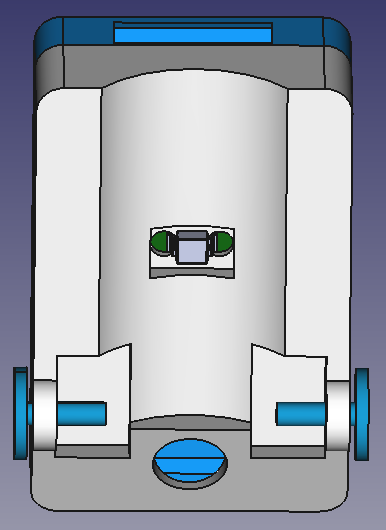
\includegraphics[width=0.45\textwidth]{../common/enc/top_base.png}}
			\hfill
			\subfloat[Spacers for pcb
			]{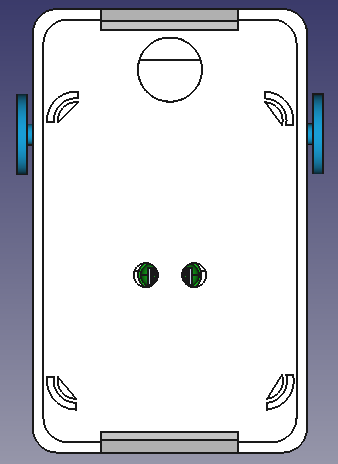
\includegraphics[width=0.45\textwidth]{../common/enc/top_base2.png}}
			\caption{Top Base}
		\end{figure}
	
	
		\begin{figure}[ht!]
			\centering
			\subfloat[Battery compartment
			]{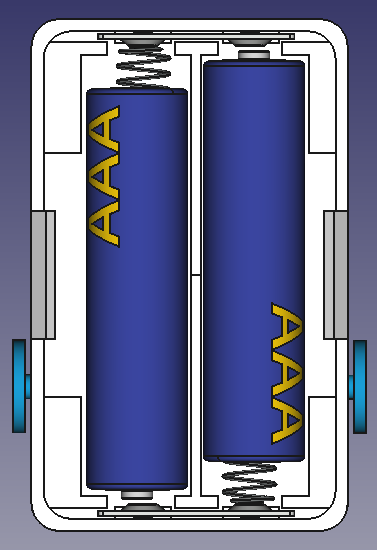
\includegraphics[width=0.45\textwidth]{../common/enc/bot_base.png}}
			\hfill
			\subfloat[Led compartment
			]{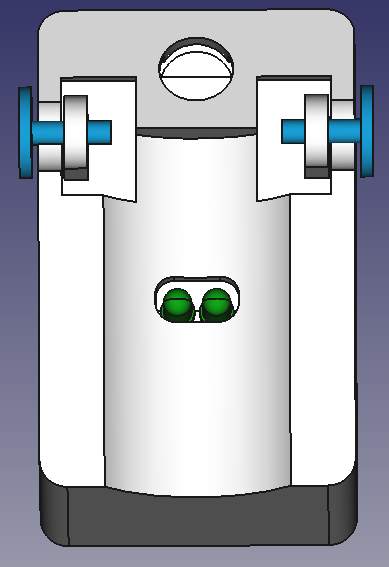
\includegraphics[width=0.45\textwidth]{../common/enc/bot_base2.png}}
			\caption{Bottom Base}
		\end{figure}
	
	
		Securing finger is an important part as any wobble or improper contact would lead to degradation in signal quality and calculated parameters. To achieve a firm pressure onto the finger which would hold it stable in place, a safety pin was used (removing the clip part) in the rotation mechanism.
		
		\begin{figure}[ht!]
			\centering
			\subfloat[Safety pin
			]{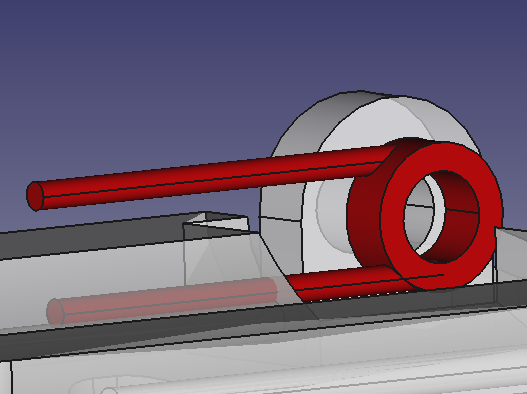
\includegraphics[width=0.5\textwidth]{../common/enc/pin.png}}
			\hfill
			\subfloat[Side view of pin
			]{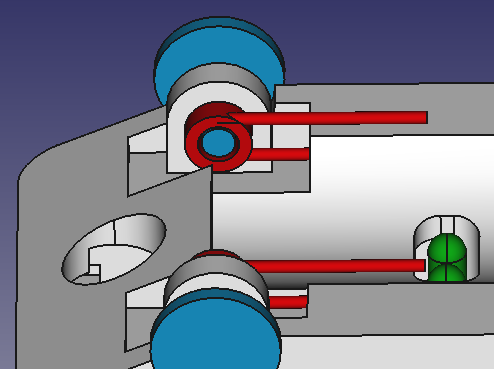
\includegraphics[width=0.5\textwidth]{../common/enc/pin_side.png}}
			\caption{Pin mounted in bottom base}
		\end{figure}	
		
		In idle position, pin would be in natural non-extended state hence both base parts would be closed. When a finger is inserted, lid needs to go up via the rotational mechanism as that is the only path to accommodate the finger. This would cause the upper part connected with pin to push down on finger which would lead to a firm grip to form ensuring good contact with photodiode and led.

		\begin{figure}[ht!]
			\centering
			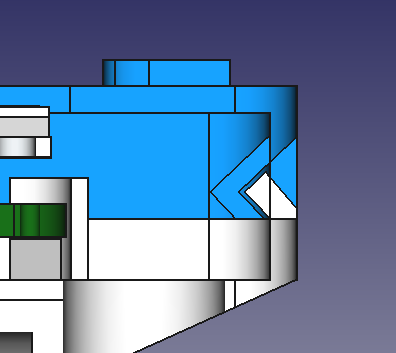
\includegraphics[width=0.6\textwidth]{../common/enc/snap.png}
			\caption{Snap fit cross-section}
		\end{figure}	
		
	
		Snap fit elements were implemented making it easier to fit and remove the cover parts whenever required.

	\pagebreak
	
	
	\begin{thebibliography}{10}		
		\begin{english}
			
		\bibitem{light}
		Hartmann Vera, Liu Haipeng.
		\textit{Quantitative Comparison of Photoplethysmographic 
			Waveform Characteristics: Effect of Measurement Site}
		Frontiers in Physiology , vol 10 (2019)
		\url{https://www.frontiersin.org/article/10.3389/fphys.2019.00198}
		
		\bibitem{penetrate}
		Ash, Caerwyn et al.
		\textit{Effect of wavelength and beam width on 
			penetration in light-tissue interaction using computational methods.}
		Lasers in medical science vol. 32,8 (2017): 1909-1918.
		\url{https://www.ncbi.nlm.nih.gov/pmc/articles/PMC5653719/}		
		
		\bibitem{skin}
		Feiner, John R. MD, Severinghaus.
		\textit{Dark Skin Decreases the Accuracy of Pulse Oximeters at 
			Low Oxygen Saturation}
		December 2007 - Volume 105 - Issue 6 - p S18-S23
		\url{https://journals.lww.com/anesthesia-analgesia/Fulltext/2007/12001/Dark_Skin_Decreases_the_Accuracy_of_Pulse.4.aspx}		
		
		\bibitem{mmpd} 
		Argüello-Prada, Erick Javier. 
		\textit{The mountaineer's method for peak detection in photoplethysmographic signals.} 
		Revista Facultad De Ingenieria-universidad De Antioquia 2018 (2019): 42-50
		\url{https://api.semanticscholar.org/CorpusID:116767900}
		
		\bibitem{nxp} 
		Santiago Lopez, Freescale Semiconductor.
		\textit{Pulse Oximeter Fundamentals and Design} 
		Document Number: AN4327, Rev. 2, 11/2012
		\url{https://www.nxp.com/docs/en/application-note/AN4327.pdf}
		
		\bibitem{ti}
		Praveen Aroul, Texas Instruments.
		\textit{Miniaturized Pulse Oximeter Reference Design}
		User’s Guide and Test Report TIDA-00311
		\url{https://www.ti.com/lit/pdf/tidu542}
		
		\bibitem{micro}
		Zhang Feng, Microchip Technology Inc.
		\textit{Pulse Oximeter Design Using Microchip’s Analog Devices
			and dsPIC® Digital Signal Controllers (DSCs)}
		AN1525,   04/28/2015
		\url{http://ww1.microchip.com/downloads/en/Appnotes/00001525B.pdf}
		
		\bibitem{oxf}
		Dr. Neil Townsend, Department of Engineering Science, University of Oxford.
		\textit{C3B Medical Electronics Lecture Notes}
		\url{https://www.robots.ox.ac.uk/~neil/teaching/lectures/med_elec/notes6.pdf}	
		
		\bibitem{wuk}
		Michael W. Wukitsch, BA,Michael T. Petterson.
		\textit{Pulse Oximetry: Analysis of Theory,Technology and Practice}
		\url{https://doi.org/10.1007/BF01617328}	
			
		\end{english}	
	\end{thebibliography}

	\pagebreak
	\section{समापन टिप्पणियाँ}

	मैंने पूरी प्रक्रिया के दौरान विशेष रूप से \cite{nxp}, \cite{ti}, \cite{micro}, \cite{oxf}, \cite{wuk} दस्तावेजों का व्यापक रूप से अध्ययन किया था कमियों को दूर करने और डिजाइन में सुधार/पुनरीक्षण करने के लिए।\par
	\bigskip
	
	इस प्रोजेक्ट को पूरा करने से मुझे एक डिजाइन के नज़रिए से बहुत सी चीजें सीखने को मिली और साथ हि उन उत्पादों के लिए बहुत सम्मान बडा जिनका मैं रोज उपयोग करता हूं, जाहा बड़ी संख्या में मापदंडों को जाँचा जाता है और यह सुनिश्चित किया जाता है कि प्रोडक्ट सही काम करता हो। 	
	
	य़ह प्रोजेक्ट बनाने मे मुझे 7 महिने लगे और औसत 20 घंटे प्रति हफ्ता काम किया इस पर। इस दौरान मेने 3 वर्जन बनाये, यह लेख तीसरे वर्जन पर आधारित है। इस वर्जन मे और भि सुधार किया जा सक़ता है इसीलिये प्रोजेक्ट डायरेक्टरी मे एक लिखन मौजूद है जाहा सारे सुधारो और मोजूदा कमियों को लिखा गया है। मे इन पर आगे काम नही करना चाहूंगा क्योँकि जिन कारणों से इस प्रोजेक्ट को शुरु किया था, उनकी पुरती हो गई है:
	
	\begin{itemize}
		\item एक प्रोजेक्ट सम्भालना और उसे शुरु से अंत तक खत्म करना। साथ हि 2 भाशाओ मे इसका लेखन करना। 
		\item प्रोजेक्ट का एक YouTube व्लॉग। 
	\end{itemize}
	
	मैंने अतीत में इनमें से कुछ भी नहीं किया था इसलिए इस परियोजना को पूरा करने के लिए मुझे खुद को बदलने की आवश्यकता थी। इस यात्रा से मैंने जो सबसे महत्वपूर्ण सबक सीखे हैं वे हैं:
	
	\begin{itemize}
		\item कभी भी किसी ऐसी चीज को जो मुश्किल या पहुंच से बाहर लगती है, उस पर काम करने के अपने निर्णय पर विचार न करना। आप कुछ भी नहीं जानते हैं, इसलिए सब कुछ मुश्किल होगा, लेकिन यह मुश्किल, किसी काम को करने के चुनाव का आधार नही बननी चाहिये।
		
		\item संगतता। डिज़ाइन के साथ कई मुद्दे थे जो मुझे सप्ताहांत पर मिले, जो बाद में अगले सप्ताहांत में हल हो गए, क्योंकि इसमें निरंतरता थी और मैं हर दिन उस समस्या से जुड़ा था।
		
	\end{itemize}
	
	\bigskip
	मैं अब इस दस्तावेज़ को समाप्त करता हूँ। यदि आपके पास कोई सुझाव या टिप्पणी है, तो आप मुझसे Twitter \href{https://twitter.com/yskabhijeet}{@yskabhijeet} पर संपर्क कर सकते हैं। 

	
\end{document}